\scanpage{25}

Le Lemme 4 nous ramène
alors à vérifier le

\uline{Lemme 5} (\unsure{notations} comme le th).

Sous les conditions du th, mais
sans \deleted{\unsure{supposer} \illegible{3}}
\inserted{supposer $\unsure{y_0|Y}$ \deleted{\unsure{géom.}} \uline{unibranche}}
en $y_0$, \inserted{ni $f$ propre,} pour tt pt fermé \inserted{$x$} de $X_0$,
\deleted{l'anneau local} $\operatorname{Spec}(\unsure{\widehat{\underline O}|\underline O}_{X_0,x})$ est
connexe en dim $\geq h$

\margin{\unsure{Bien plutôt} : tout $x$ tel que $\dim\bar x<h$,
$(\operatorname{Spec}\underline{O}_{X_0,x})'$ est connexe}

En effet, le lemme 1 \inserted{\figure{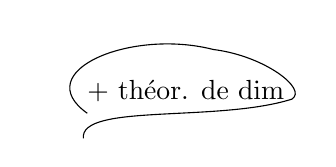
\begin{tikzpicture}[x=1cm,y=1cm]
\node at (0,0) {+ \unsure{théor. de dim}};
\draw (-1.25,-.28) .. controls (-2,.25) and (-.7,.8) .. (.35,.53)
.. controls (1,.45) and (1.55,.03) .. (1.35,-.1)
.. controls (.4,-.4) and (-1.35,-.15) .. (-1.3,-.6);
\end{tikzpicture}}} nous
ramène facilement, utilisant
l'hypothèse sur $X_1$, au cas où
$X_0$ est \uline{irréductible} \deleted{de dim $\geq h+1$},
donc $X$ \uline{irréductible} dominant $Y$,
\inserted{donc $=$ intègre comme $Y$.}
On peut supposer par une réduction
facile (?) au cas où
\deleted{``le \unsure{complété de} \illegible{2}}
\inserted{$\underline{O}_{Y,y_0}$ est}
\inserted{\unsure{formellt} équidimensionnel}
\deleted{\unsure{dimensions} \illegible{2} pour $\underline{O}_{Y,y_0}$''.}
\margin{conjecture}

D'où
\[
\dim\underline{O}_{X,x}
=\underbrace{\dim\underline{O}_{Y,y_0}}_{n}
+\underbrace{\dim X_1}_{\geq h+1}
\]

\margin{24}
